\documentclass{article}
\usepackage{enumitem}
\usepackage[cachedir=minted_cache]{minted}
\usepackage{graphicx}
\graphicspath{ {./img/} }
\usepackage[margin=1in]{geometry} %used to set the margins
\setcounter{secnumdepth}{0} %used to get rid of section numbers
\title{Lab 11: Graph Algorithms}
\author{Michael Morikawa}
\date{\today}


\begin{document}
\maketitle
\section{Lab Questions}
\begin{enumerate}[label=\textbf{Question \arabic*}]
      \item  Does Dijkstra's algorithm perform a DFS or BFS on a graph? Explain. \\
            \textbf{
                  It is pretty close to doing a BFS on the graph, since it considers
                  the vertices adjacent to whatever vertex it is at. However, the next vertex
                  that is processed is not the next one on the same level or the first in the next level;
                  what gets processed next is the vertex with the current shortest distance from the source
                  vertex.
            }
      \item Lab question 2: Explain the concept of “Transitive Closure” on a digraph. Provide a
            reason for performing a transitive closure on a digraph. \\
            \textbf{
                  Transitive closure is the process of connecting vertices that have a path between them by
                  adding a new edge into the graph that connects the two. A reason for performing transitive
                  closure on a graph is whenever you are only concerned with whether or not you could reach
                  a certain vertex from another. For example, this could be used to find if there are a series
                  of one or more flights to get from A to B.
            }


\end{enumerate}

\section{Source Code}

\subsection{main.cpp}
\inputminted{c++}{../src/main.cpp}

\section{Output}
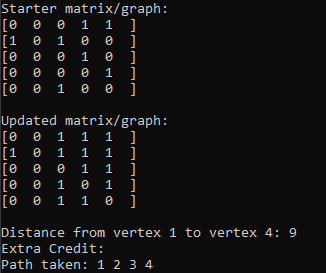
\includegraphics[]{output.png}

\end{document}